%%%%%%%%%%%%%%%%%%%%%%%%%%%%%%%%%%%%%%%%%%%%%%%%%%%%%%%%%%%%%%%%%%%%
%% I, the copyright holder of this work, release this work into the
%% public domain. This applies worldwide. In some countries this may
%% not be legally possible; if so: I grant anyone the right to use
%% this work for any purpose, without any conditions, unless such
%% conditions are required by law.
%%%%%%%%%%%%%%%%%%%%%%%%%%%%%%%%%%%%%%%%%%%%%%%%%%%%%%%%%%%%%%%%%%%%

\documentclass[
  digital,     %% The `digital` option enables the default options for the
               %% digital version of a document. Replace with `printed`
               %% to enable the default options for the printed version
               %% of a document.
%%  color,       %% Uncomment these lines (by removing the %% at the
%%               %% beginning) to use color in the printed version of your
%%               %% document
  oneside,     %% The `oneside` option enables one-sided typesetting,
               %% which is preferred if you are only going to submit a
               %% digital version of your thesis. Replace with `twoside`
               %% for double-sided typesetting if you are planning to
               %% also print your thesis. For double-sided typesetting,
               %% use at least 120 g/m² paper to prevent show-through.
  nosansbold,  %% The `nosansbold` option prevents the use of the
               %% sans-serif type face for bold text. Replace with
               %% `sansbold` to use sans-serif type face for bold text.
  nocolorbold, %% The `nocolorbold` option disables the usage of the
               %% blue color for bold text, instead using black. Replace
               %% with `colorbold` to use blue for bold text.
  lof,         %% The `lof` option prints the List of Figures. Replace
               %% with `nolof` to hide the List of Figures.
  lot,         %% The `lot` option prints the List of Tables. Replace
               %% with `nolot` to hide the List of Tables.
]{fithesis4}
%% The following section sets up the locales used in the thesis.
\usepackage[resetfonts]{cmap} %% We need to load the T2A font encoding
\usepackage[T1,T2A]{fontenc}  %% to use the Cyrillic fonts with Russian texts.
\usepackage[
  main=english, %% By using `czech` or `slovak` as the main locale
                %% instead of `english`, you can typeset the thesis
                %% in either Czech or Slovak, respectively.
  english, german, czech, slovak %% The additional keys allow
]{babel}        %% foreign texts to be typeset as follows:
%%
%%   \begin{otherlanguage}{german}  ... \end{otherlanguage}
%%   \begin{otherlanguage}{czech}   ... \end{otherlanguage}
%%   \begin{otherlanguage}{slovak}  ... \end{otherlanguage}
%%
%%
%% The following section sets up the metadata of the thesis.
\thesissetup{
    date        = \the\year/\the\month/\the\day,
    university  = mu,
    faculty     = fi,
    type        = mgr,
    department  = Department of Computer Systems and Communications,
    author      = Bc. Šimon Vacek,
    gender      = m,
    advisor     = {RNDr. Samuel Pastva, Ph.D.},
    title       = {Breadth-first-search parallelization of Binary Decision Diagrams in Rust},
    TeXtitle    = {Breadth-first-search parallelization of Binary Decision Diagrams in Rust},
    keywords    = {BDD, parallelization, concurrency, TODO ...},
    TeXkeywords = {BDD, parallelization, concurrency, TODO \ldots},
    abstract    = {
        In formal verification, a widely used representation is a Binary Decision Diagram. This directed acyclic graph allows manipulation of Boolean functions.

        This data structure typically contains a large number of nodes, on the order of thousands, even tens of millions. Operations on such a large graph are very time-consuming. There are many libraries that offer BDD solutions, but only a few multi-threaded implementations.
        
        In this Thesis, we will explore the design of a concurrent BDD implementation. // TODO
    },
    thanks      = {%
      I would like to thank my supervisor, RNDr. Samuel Pastva, Ph.D., for his leadership and support TODO...
    },
    bib         = bibliography.bib,
    %% Remove the following line to use the JVS 2018 faculty logo.
    facultyLogo = fithesis-fi,
}
\usepackage{makeidx}      %% The `makeidx` package contains
\makeindex                %% helper commands for index typesetting.
%% These additional packages are used within the document:
\usepackage{paralist} %% Compact list environments
\usepackage{amsmath}  %% Mathematics
\usepackage{amsthm}
\usepackage{amsfonts}
\usepackage{url}      %% Hyperlinks
\usepackage{markdown} %% Lightweight markup
\usepackage{listings} %% Source code highlighting
\lstset{
  basicstyle      = \ttfamily,
  identifierstyle = \color{black},
  keywordstyle    = \color{blue},
  keywordstyle    = {[2]\color{cyan}},
  keywordstyle    = {[3]\color{olive}},
  stringstyle     = \color{teal},
  commentstyle    = \itshape\color{magenta},
  breaklines      = true,
}
\usepackage{floatrow} %% Putting captions above tables
\floatsetup[table]{capposition=top}
\floatsetup[algorithm]{style=ruled,capposition=top}

\usepackage{algpseudocode}
\makeatletter %% Gemini generated to correct algorithm line referencing
\let\old@ALG@step\ALG@step
\renewcommand{\ALG@step}{%
  \old@ALG@step
  \protected@edef\@currentlabel{\theALG@line}%
}
\makeatother

\floatstyle{ruled}
\newfloat{algorithm}{htbp}{loa}
\floatname{algorithm}{Algorithm}
\usepackage[babel]{csquotes} %% Context-sensitive quotation marks
\begin{document}
%% The \chapter* command can be used to produce unnumbered chapters:
\chapter*{Introduction}
%% Unlike \chapter, \chapter* does not update the headings and does not
%% enter the chapter to the table of contents. If we want correct
%% headings and a table of contents entry, we must add them manually:
\markright{\textsc{Introduction}}
\addcontentsline{toc}{chapter}{Introduction}

BDDs are pretty cool, but heavy on the computation, here are top 3 reasons why: // TODO


\chapter{Binary Decision Diagrams}
\label{chap:bdd}

A Binary Decision Diagram (BDD) is an abstract data type representing a Boolean function, offering convenient creation,
manipulation, and analysis of Boolean functions in symbolic form \cite{bdds}. A BDD is a directed acyclic graph
structure widely used in formal design verification, test generation, and logic synthesis that provides an algorithmic
basis for symbolic model checkers \cite{bfs-bdd, bdds}.

A BDD is a collection of nodes (or vertices) interconnected with each other by links (or edges). In a BDD, leaf nodes
are called terminal nodes, labeled with Boolean values 0 and 1. The non-terminal nodes are referred to as inner nodes.
Each inner node is labeled with a Boolean variable $x_i$. An inner node has exactly two outgoing links: a low link and
a high link. When traversing the BDD, the chosen link depends on the valuation of $x_i$, $v(x_i)$. A low link
corresponds to $v(x_i)=0$ while high link to $v(x_i)=1$.

A simple BDD representing a single variable $x$ is depicted in Figure \ref{fig:simple-bdd}. The BDD contains two
terminal nodes $0$ and $1$, which are portrayed as square nodes. As a convention, all inner nodes use circles. In this
case, there is a single inner node with variable $x$. The high links are marked with a solid line and low links with a
dashed line. For $v(x) = 0$, the low link is followed to the corresponding terminal node $0$.

\begin{figure}
    \centering
    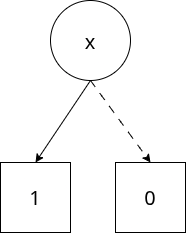
\includegraphics[width=0.2\linewidth]{figures/simple-bdd.png}
    \caption{The simplest BDD of a function $f(x)=x$}
    \label{fig:simple-bdd}
\end{figure}

Consider the following Boolean function:
\begin{equation}
    \label{eq:example}
    f(x_1, x_2, x_3) = (x_1 \land x_2) \lor x_3
\end{equation}
Function $f$ performs AND and OR on a vector of variables $X=(x_1, x_2, x_3)$. An example of a BDD representing this
function is portrayed in Figure \ref{fig:bdd}. In this case, the root node contains $x_2$. This particular BDD has
three interesting properties:

\begin{enumerate}
    \item Following only the high links from the root node, we will encounter an $x_3$ node with both of its
        links directed to the terminal node $1$. Similarly, the low link of $x_2$ also has both links directed to the
        same node. These are called \textit{redundant nodes}. \label{item:redundancy}
    \item There are two $x_3$ nodes with links to the terminal node $0$ and $1$. These are identical. Just like the
        two pairs of terminal nodes. \label{item:duplicate}
    \item The root node's high and low successors are $x_1$ and $x_3$ respectively. Following the low link leads to
        the aforementioned node $x_3$, which is again followed by node $x_3$. \label{item:ordering}
\end{enumerate}

While the BDD is correct, the graph is hard to read. Furthermore, these properties create implementation challenges
and increase both time and space complexity for the operations performed on this data structure. The point
\ref{item:ordering} outlines variables scattered in a seemingly random order. This makes the layer-by-layer
Breadth-first processing more challenging. To address this, let's consider an \textit{Ordered Binary Decision
Diagram} (OBDD).

\begin{figure}
    \centering
    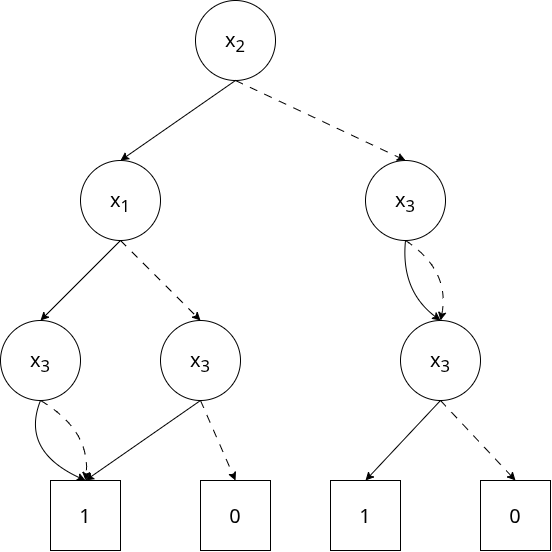
\includegraphics[width=0.6\linewidth]{figures/example-bdd.png}
    \caption{Binary Decision Diagram representing Boolean function $(x_1 \land x_2) \lor x_3$.}
    \label{fig:bdd}
\end{figure}

An OBDD enforces a fixed variable ordering restriction. Let's assume a total ordering of variables
$x_n < x_n+1 < \ldots < x_{n+k}$ where the variable of terminal nodes in this ordering is assumed to be $\infty$,
so that $\infty > x_{n+k}$ \cite{ruddy}. A fixed variable ordering guarantees that traversing the BDD encounters the
variables in a certain order. This new property allows the graph to be structured level-by-level with a level per each
variable. This enables level-wise memory management and breadth-first manipulation algorithms \cite{bfs-bdd, oxidd}.

Figure \ref{fig:obdd} displays the function $f$ of (\ref{eq:example}) as an OBDD with the previously stated variable
ordering. It is evident that nodes with variables $x_1$ and $x_2$ have swapped places, but also the redundant node
with $x_3$ was eliminated as the ordering $x_3 \nless x_3$ was violated.


\begin{figure}
    \centering
    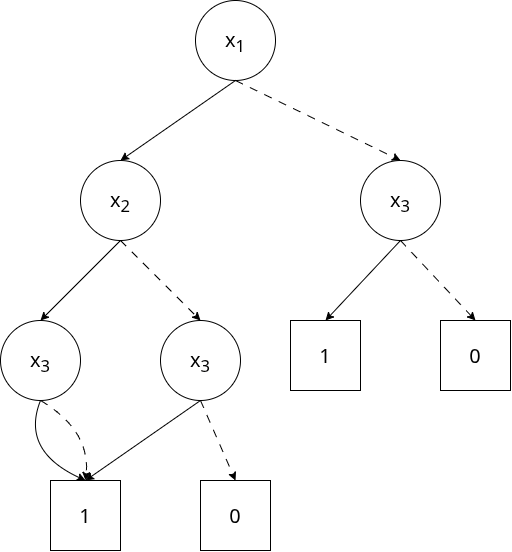
\includegraphics[width=0.6\linewidth]{figures/example-obdd.png}
    \caption{Ordered Binary Decision Diagram representing Boolean function $(x_1 \land x_2) \lor x_3$.}
    \label{fig:obdd}
\end{figure}

As per points \ref{item:redundancy} and \ref{item:duplicate}, these are eliminated with further restrictions applied
to an OBDD. A \textit{Reduced Ordered Binary Decision Diagram} (ROBDD) is defined by the following rules:
\begin{itemize}
    \item There are no redundant nodes. Such is a node $a$ that $high(a) = low(a)$
    \item There are no duplicate nodes. Nodes $a$ and $b$ are duplicates if:
    \begin{itemize}
        \item $var(a) = var(b)$
        \item $high(a) = high(b)$
        \item $low(a) = low(b)$
    \end{itemize}
\end{itemize}
The ROBDD is a canonical form for Boolean functions \cite{bdds-bryant}. That is, for a given variable ordering, every
Boolean function over these variables has a unique (up to isomorphism) representation as a reduced OBDD \cite{bdds}.
The greatest advantage of this representation is its compactness, which reduces the memory footprint, as well as
testability for correctness in libraries.

The ROBDD representation of our example OBDD is in Figure \ref{fig:robdd}. The redundant node with $x_3$ was
removed, and the other $x_3$ nodes were merged into one. Had we chosen a different variable ordering, for example 
$x_n > x_n+1 > \ldots > x_{n+k}$, the ROBDD would be the one displayed in Figure \ref{fig:robdd-reordered}.

\begin{figure}
    \centering
    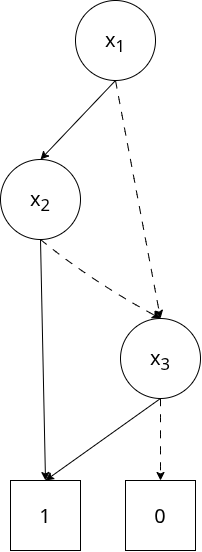
\includegraphics[width=0.22\linewidth]{figures/example-robdd.png}
    \caption{Reduced Ordered Binary Decision Diagram representing Boolean function $(x_1 \land x_2) \lor x_3$.}
    \label{fig:robdd}
\end{figure}

\begin{figure}
    \centering
    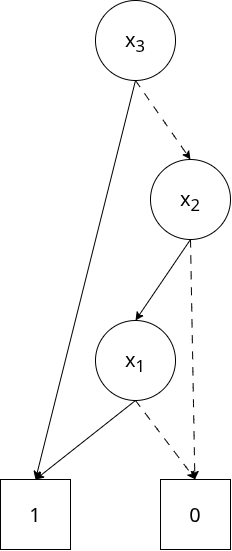
\includegraphics[width=0.25\linewidth]{figures/example-robdd-reordered.png}
    \caption{Reduced Ordered Binary Decision Diagram representing Boolean function $(x_1 \land x_2) \lor x_3$ with variable
    ordering reversed to the one of \ref{fig:robdd}.}
    \label{fig:robdd-reordered}
\end{figure}

There are other BDD types with further restrictions or modified properties, such as a \textit{Multi Terminal
BDD} (MTBDD), which  allows for additional leaf nodes, besides $0$ and $1$, or \textit{Multi-valued DD} (MDD)
which is a generalization of a BDD to other domains beyond the Boolean domain \cite{sylvan}. All of these types are,
however, outside the scope of this Thesis. The remainder of this text focuses exclusively on ROBDD. The terms BDD and
ROBDD will be used interchangeably from this point forward.


\section{The Apply operation}
\label{chap:bdd:apply}

A BDD is a convenient representation for satisfiability testing, equivalence checking, and performing Boolean
operations on them. Applying a Boolean operation (such as AND, OR, XOR) on two BDDs is one of the key operations of
the BDD interface \cite{bfs-bdd}. This operation, referred to as \textit{apply}, is the primary focus of this Thesis.
$apply$ takes three arguments: two BDDs and the Boolean operation. The product is then also a BDD. To better illustrate
this, consider these Boolean functions:

\begin{alignat}{1}
     f(x_1, x_2) &= x_1 \lor x_2 \label{eq:apply-a} \\
     g(x_1, x_3) &= x_1 \lor x_3 \label{eq:apply-b} \\
               h &= f \land g \label{eq:apply-result}
\end{alignat}

Function $h$ in \eqref{eq:apply-result} is the product of applying the conjunction operation to functions $f$ and $g$.
After substituting $f$ and $g$ for their definitions and simplifying the expression, we are left with 
$h(x_1, x_2, x_3) = x_1 \lor (x_2 \land x_3)$. In terms of BDD, this operation is illustrated in Figure
\ref{fig:apply}.

\begin{figure}
    \centering
    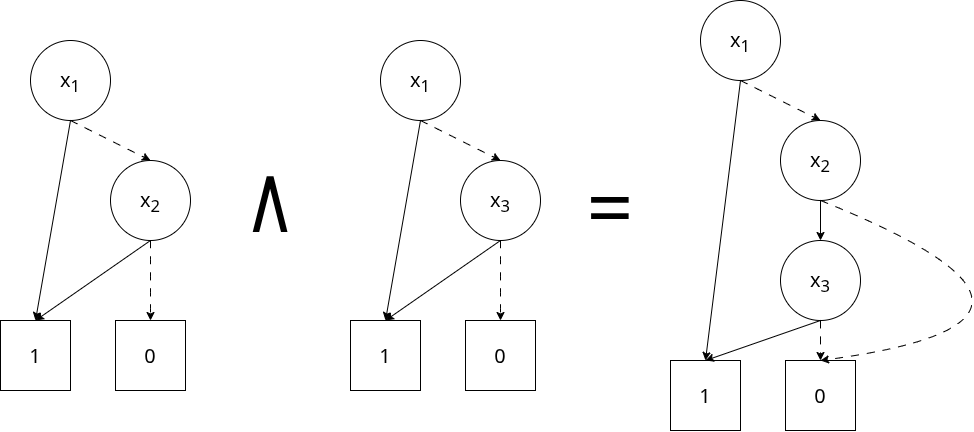
\includegraphics[width=\linewidth]{figures/example-apply.png}
    \caption{ROBDD produced by apply, as shown in \eqref{eq:apply-result}}
    \label{fig:apply}
\end{figure}

Most commonly, $apply$ is implemented with the use of recursion, which happens to be easier to demonstrate. Algorithm
\ref{alg:apply} presents the pseudocode of the $apply$ operation. $apply$ returns the root node of the resulting BDD and
takes three arguments:
\begin{enumerate}
    \item A root node of the first BDD
    \item A root node of the second BDD
    \item A Boolean operation, e.g. conjunction
\end{enumerate}

Both BDDs are traversed simultaneously in a depth-first manner from the top to the terminal nodes. Each recursive algorithm
has a base condition to stop the recursion; in this case, it is when a terminal node of each BDD is reached. On line
\ref{alg:apply:recursion-stop}, both of the nodes are used as arguments to the $op$ operation, and the result is returned to
the previous call in the call stack.

If neither or only one of the current nodes is terminal, the task cache is checked on line \ref{alg:apply:cache-get}. This
check prevents repeated computation of results that were already processed. A task cache is a commonly used optimization that
reduces the complexity class of many BDD operations from exponential time to polynomial time \cite{sylvan}.

For node pairs that have not been encountered before (or whose result was replaced due to use of a lossy cache), the algorithm
chooses a path to progress. Line \ref{alg:apply:min-var} determines which BDD to expand further, for only the BDD with a
lower variable is progressed (assuming the standard variable ordering). After the low and high node pairs of both BDDs are
assigned, the $apply$ function is called recursively for both successors (lines \ref{alg:apply:apply-l} and
\ref{alg:apply:apply-h}).

Once both the low and high successors are known, the new resulting node can be created. To keep the resulting BDD still
reduced, redundant and duplicate nodes need to be eliminated. The $if$ statement on line $\ref{alg:apply:redundancy-check}$
enforces the redundancy rule. The function $ensure\_node$ called on line \ref{alg:apply:ensure-node} serves two purposes:
\begin{itemize}
    \item Create a new node for the given variable $v$, low successor $l$ and high successor $h$
    \item Check for duplicities and create this node if and only if it is unique to the BDD. Return an existing node otherwise
\end{itemize}

The final steps of the algorithm are to store the result in the task cache and return the result node. Calling $apply$ with
two root nodes and an operation yields a root node of the calculated BDD.

\begin{algorithm}
    \caption{Apply}\label{alg:apply}
    \begin{algorithmic}[1]
        \Require $node\_a$ a root node of BDD $a$
        \Require $node\_b$ a root node of BDD $b$
        \Require $op$ a Boolean operation
        \Ensure $c$ a root node of the resulting BDD
        \Function{apply}{$node\_a, node\_b, op$}
            \If{$node\_a$ is terminal AND $node\_b$ is terminal} \label{alg:apply:recursion-stop}
                \State \Return  $op(node\_a, node\_b)$
            \EndIf
            \State $chached\_res \gets cache.get(node\_a, node\_b, op)$
            \If{$cached\_res \neq null$} \label{alg:apply:cache-get}
                \State \Return $cached\_res$
            \EndIf
            \State $v \gets min(var(node\_a), var(node\_b))$ \label{alg:apply:min-var}
            \If{$var(node\_a) = v$}
                \State $(low\_a, high\_a) \gets (low(node\_a), high(node\_a))$
            \Else
                \State $(low\_a, high\_a) \gets (node\_a, node\_a)$
            \EndIf
            \If{$var(node\_b) = v$}
                \State $(low\_b, high\_b) \gets (low(node\_b), high(node\_b))$
            \Else
                \State $(low\_b, high\_b) \gets (node\_b, node\_b)$
            \EndIf
            \State $l \gets apply(low\_a, low\_b)$ \label{alg:apply:apply-l}
            \State $h \gets apply(high\_a, high\_b)$ \label{alg:apply:apply-h}
            \If{$l \neq h$}A \label{alg:apply:redundancy-check}
                \State $c \gets ensure\_node(v, l, h)$ \label{alg:apply:ensure-node}
            \Else
                \State $c \gets l$
            \EndIf
            \State $cache.put(node\_a, node\_a, op, c)$
            \State \Return $c$
        \EndFunction
    \end{algorithmic}
\end{algorithm}

The recursive approach is fairly easy to understand and implement. In practice, however, recursive algorithms print long stack
traces and can be harder to debug, so it is not always desirable. It also reduces possibilities for parallel execution, the
main focus of this Thesis. Alternatively, recursion can be eliminated in favor of iterative computation with supporting data
structures. We will explore this more in the following subsection.

\subsection{DFS vs BFS}
\label{chap:bdd:apply:dfs-bfs}

- dfs uses a stack

- bfs uses a queue

This is the operation in the focus of this Thesis. The aim of this Thesis is to explore and assess a parallel approach using BFS. For this reason, only one Boolean operation is implemented - conjunction.


\chapter{Approaches to BDD parallelization}

All found concurrent implementations of BDD implement a recursive approach to depth-first traversal \cite{oxidd, sylvan}. 


\chapter{Design}
\label{chap:design}

We will focus on implementing a Shared Binary Decision Diagram, a multi-rooted directed acyclic graph that represents multiple Boolean functions \cite{bfs-bdd}.

\chapter{Implementation}
\label{chap:impl}


\chapter{Comparisons and benchmarks}
\label{chap:comparisons-benchmarks}


\chapter{Conclusion}

\nocite{*} %% TODO DELETEME
\printbibliography[heading=bibintoc] %% Print the bibliography.


\appendix %% Start the appendices.
\chapter{An appendix}
Here you can insert the appendices of your thesis.

\end{document}
